\documentclass{article}%
\usepackage[T1]{fontenc}%
\usepackage[utf8]{inputenc}%
\usepackage{lmodern}%
\usepackage{textcomp}%
\usepackage{lastpage}%
\usepackage{geometry}%
\geometry{margin=0.2in}%
\usepackage{graphicx}%
%
\title{Report on AustraliaWeather dataset}%
\author{Classify2TeX}%
\usepackage{amsmath}%
\usepackage{amssymb}%
\usepackage{enumitem}%
%
\begin{document}%
\normalsize%
\maketitle%
\newpage%
\tableofcontents%
\newpage%
\section{Exploratory Data Analysis}%
\label{sec:ExploratoryDataAnalysis}%
\subsection{Non{-}Null Count, Dtype of features}%
\label{subsec:Non{-}NullCount,Dtypeoffeatures}%
The table 1 provides information about the dataset, including the number of non-null values and the data types of each feature.%


\begin{table}[h!]%
\caption{Dataset Columns Information}%
\vspace{0.2cm}%
\centering%
\begin{tabular}{|c||c||c||c|}%
\hline%
Index&Column&Non{-}Null Count&Dtype\\%
\hline%
0&Date&3000&object\\%
1&Location&3000&object\\%
2&MinTemp&2961&float64\\%
3&MaxTemp&2970&float64\\%
4&Rainfall&2922&float64\\%
5&Evaporation&1667&float64\\%
6&Sunshine&1506&float64\\%
7&WindGustDir&2791&object\\%
8&WindGustSpeed&2793&float64\\%
9&WindDir9am&2787&object\\%
10&WindDir3pm&2915&object\\%
11&WindSpeed9am&2966&float64\\%
12&WindSpeed3pm&2937&float64\\%
13&Humidity9am&2939&float64\\%
14&Humidity3pm&2898&float64\\%
15&Pressure9am&2681&float64\\%
16&Pressure3pm&2684&float64\\%
17&Cloud9am&1832&float64\\%
18&Cloud3pm&1771&float64\\%
19&Temp9am&2958&float64\\%
20&Temp3pm&2918&float64\\%
21&RainToday&2922&object\\%
22&RainTomorrow&2926&object\\%
\hline%
\end{tabular}%
\end{table}

%
\newpage%
\subsection{Descriptive Statistics}%
\label{subsec:DescriptiveStatistics}%
The table 2 provides descriptive statistics for the dataset, including the count, mean, standard deviation, minimum, and maximum values.%


\begin{table}[h!]%
\caption{Dataset Descriptive Statistics}%
\vspace{0.2cm}%
\centering%
\begin{tabular}{|c||c||c||c||c||c||c||c||c||c|}%
\hline%
Index&Column Name/Statistic&count&mean&std&min&25\%&50\%&75\%&max\\%
\hline%
0&MinTemp&2961.0&11.96&6.33&{-}5.0&7.5&11.8&16.8&29.4\\%
1&MaxTemp&2970.0&22.97&7.17&{-}1.9&17.6&22.3&28.1&46.1\\%
2&Rainfall&2922.0&2.15&7.79&0.0&0.0&0.0&0.8&225.0\\%
3&Evaporation&1667.0&5.35&3.75&0.0&2.6&4.6&7.4&31.0\\%
4&Sunshine&1506.0&7.46&3.87&0.0&4.6&8.2&10.7&14.5\\%
5&WindGustSpeed&2793.0&39.81&13.33&9.0&31.0&39.0&46.0&106.0\\%
6&WindSpeed9am&2966.0&14.02&8.93&0.0&7.0&13.0&19.0&65.0\\%
7&WindSpeed3pm&2937.0&18.66&8.87&0.0&13.0&19.0&24.0&65.0\\%
8&Humidity9am&2939.0&69.13&18.85&4.0&57.0&70.0&83.0&100.0\\%
9&Humidity3pm&2898.0&51.86&20.79&4.0&37.0&52.0&66.0&100.0\\%
10&Pressure9am&2681.0&1017.89&7.12&982.2&1013.2&1017.8&1022.6&1040.3\\%
11&Pressure3pm&2684.0&1015.52&7.08&984.2&1010.6&1015.5&1020.3&1037.6\\%
12&Cloud9am&1832.0&4.49&2.88&0.0&1.0&5.0&7.0&8.0\\%
13&Cloud3pm&1771.0&4.58&2.72&0.0&2.0&5.0&7.0&8.0\\%
14&Temp9am&2958.0&16.74&6.44&{-}4.1&12.0&16.25&21.4&35.2\\%
15&Temp3pm&2918.0&21.43&6.99&{-}1.0&16.23&20.7&26.3&44.5\\%
\hline%
\end{tabular}%
\end{table}

%
\newpage%
\subsection{Distribution of features}%
\label{subsec:Distributionoffeatures}%
This section provides a visual representation of the distribution of features in the dataset using histograms (numerical features) and bar charts (categorical features). These visualizations can help in understanding the data.%
\subsubsection{Histograms of Numerical columns}%
\label{ssubsec:HistogramsofNumericalcolumns}%
The histograms below show the distribution of numerical features in the dataset.%


\begin{figure}[h!]%
\centering%
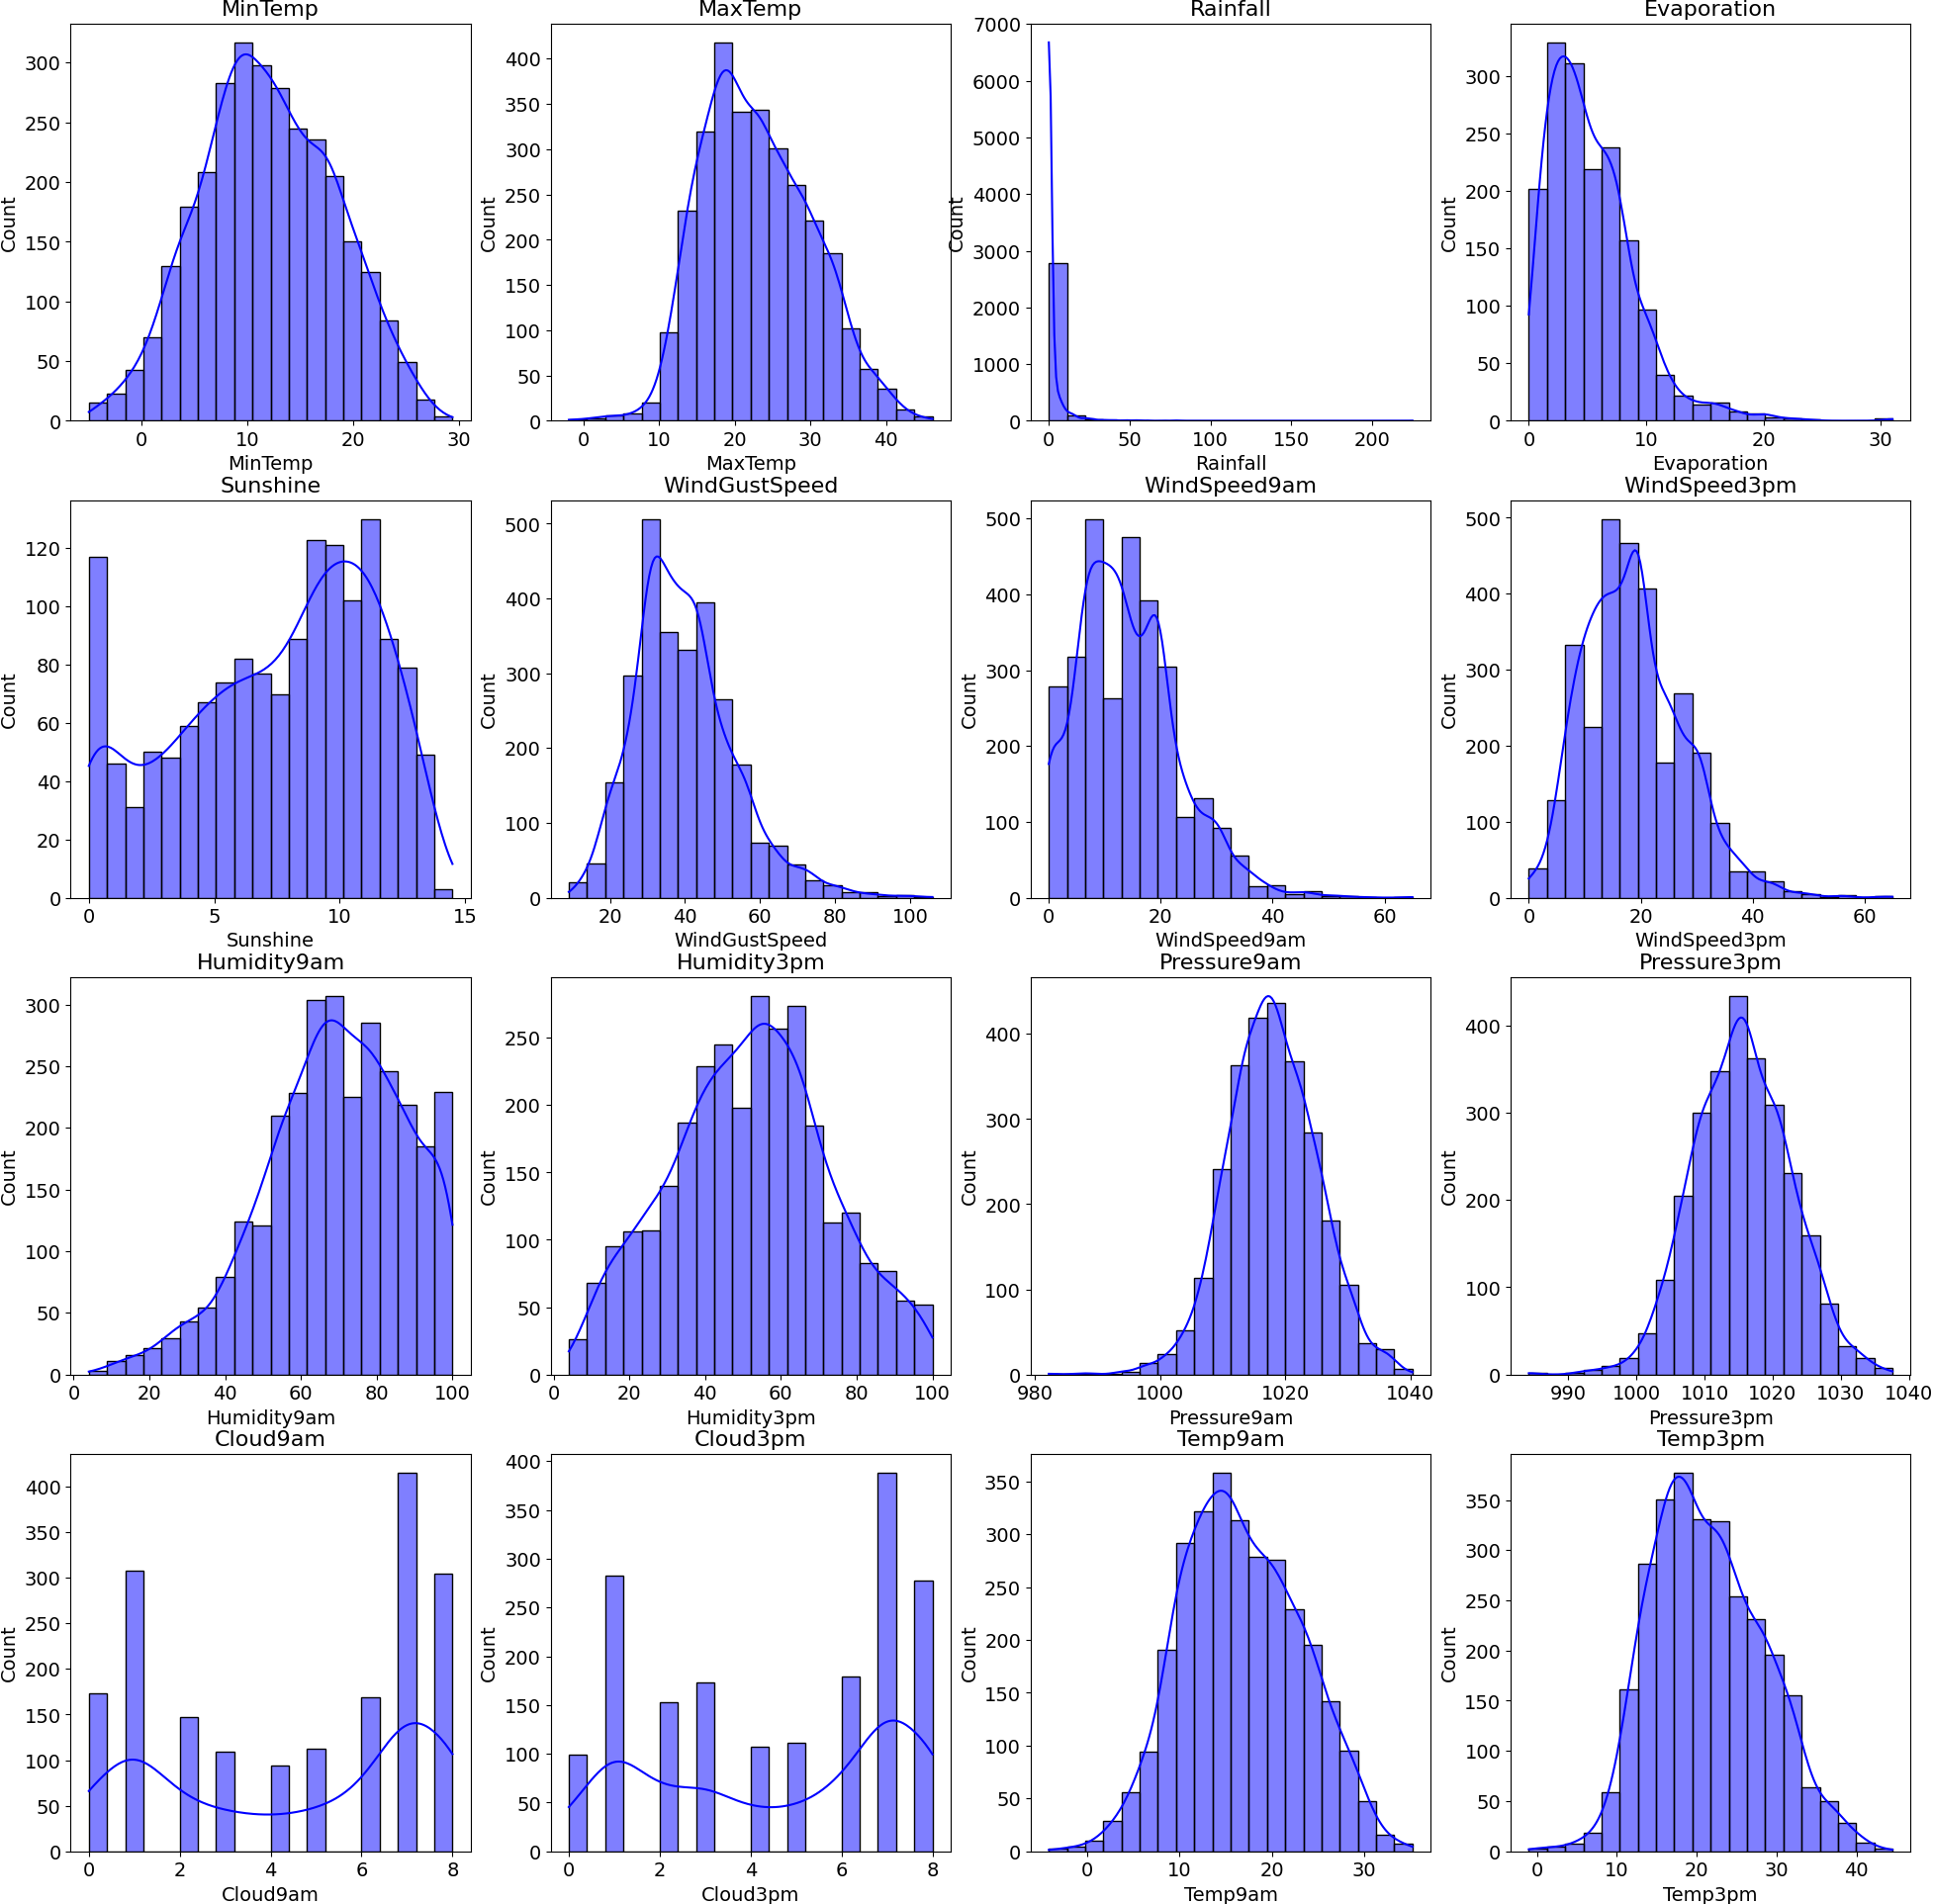
\includegraphics[width=460px]{EDA/histograms.png}%
\caption{Histograms of Numerical columns}%
\end{figure}

%
\newpage%
\subsubsection{Bar Charts of Categorical columns}%
\label{ssubsec:BarChartsofCategoricalcolumns}%
The bar charts below show the distribution of categorical features in the dataset.%


\begin{figure}[h!]%
\centering%
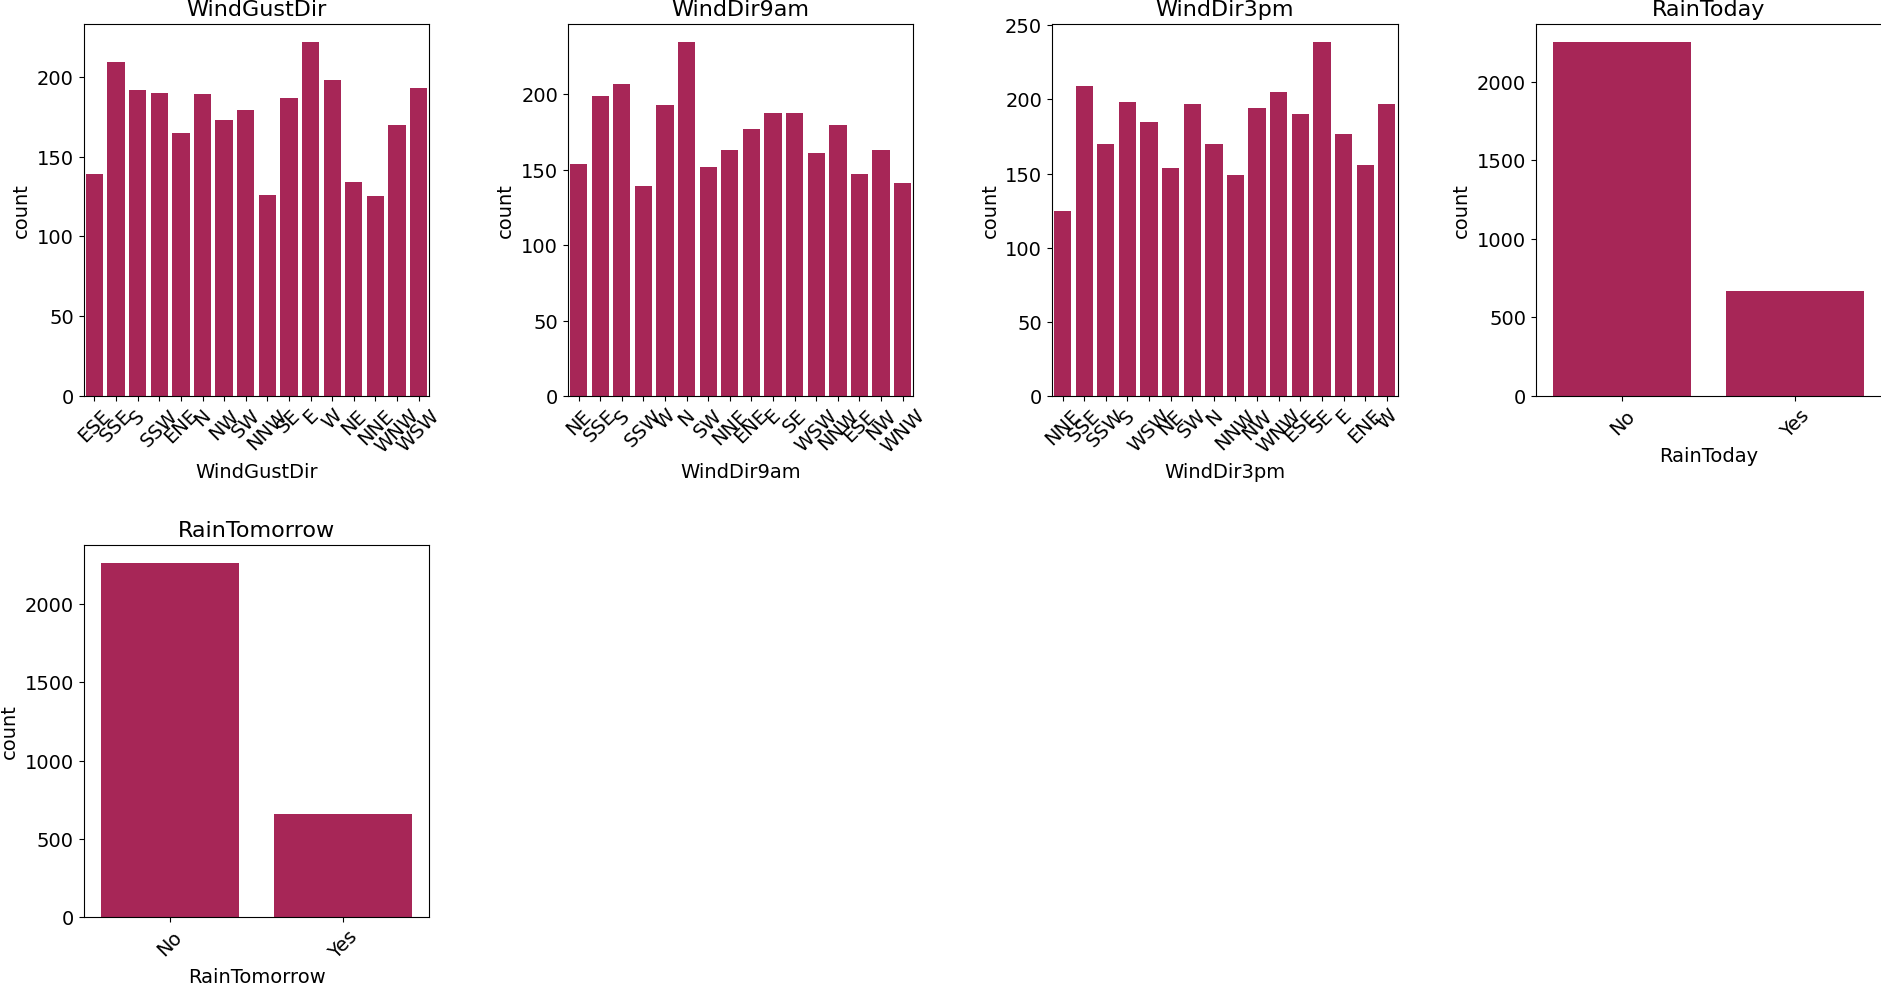
\includegraphics[width=460px]{EDA/bar_charts.png}%
\caption{Bar Charts of Categorical columns}%
\end{figure}

%
\newpage%
\section{Evaluation Metrics}%
\label{sec:EvaluationMetrics}%
\subsection{Accuracy}%
\label{subsec:Accuracy}%

                \textbf{Accuracy} is one of the simplest evaluation metrics for classification models. 
                It is defined as the ratio of correctly predicted observations to the total number of observations:

                \[
                \text{Accuracy} = \frac{\text{Number of Correct Predictions}}{\text{Total Number of Predictions}}
                \]

                While accuracy is intuitive and easy to understand, it may not be suitable for imbalanced datasets. 
                For example, in a dataset where 95\% of the samples belong to one class, predicting the majority class for every instance 
                would result in high accuracy but poor performance on the minority class.
                

%
\subsection{F1 Score}%
\label{subsec:F1Score}%

                The \textbf{F1 Score} is the harmonic mean of Precision and Recall, providing a balance between the two. 
                It is particularly useful when dealing with imbalanced datasets. Precision and Recall are defined as follows:

                \[
                \text{Precision} = \frac{\text{True Positives}}{\text{True Positives} + \text{False Positives}}
                \]
                \[
                \text{Recall} = \frac{\text{True Positives}}{\text{True Positives} + \text{False Negatives}}
                \]

                The F1 Score combines these metrics:

                \[
                \text{F1 Score} = 2 \cdot \frac{\text{Precision} \cdot \text{Recall}}{\text{Precision} + \text{Recall}}
                \]

                A high F1 Score indicates a good balance between Precision and Recall, making it a valuable metric in scenarios where false positives 
                and false negatives have significant costs.
                

%
\subsection{ROC AUC}%
\label{subsec:ROCAUC}%

                The Receiver Operating Characteristic (ROC) curve plots the True Positive Rate (Recall) against the False Positive Rate at various threshold settings. 
                The \textbf{Area Under the Curve (AUC) of the ROC curve} measures the overall ability of the model to distinguish between classes. 

                \[
                \text{AUC} = \int_{\text{FPR}=0}^{1} \text{TPR}(\text{FPR}) \, d(\text{FPR})
                \]

                Key points about ROC AUC:
                \begin{itemize}
                    \item An AUC of 0.5 indicates random guessing.
                    \item An AUC of 1.0 indicates perfect classification.
                    \item It is a threshold-independent metric, providing an aggregate measure of performance across all classification thresholds.
                \end{itemize}

                ROC AUC is particularly useful for binary classification tasks and provides insights into the trade-off between sensitivity and specificity.
                

%
\newpage%
\section{Model Optimization Results}%
\label{sec:ModelOptimizationResults}%
\subsection{Optimization Results Tables}%
\label{subsec:OptimizationResultsTables}%


\begin{table}[h!]%
\caption{Random Forest Hyperparameters and achivied metrics}%
\vspace{0.2cm}%
\centering%
\begin{tabular}{|c||c||c||c||c||c||c||c||c||c|}%
\hline%
Index&Metric/Hyperp.\textbackslash{} Iteration&0&1&2&3&4&5&6&7\\%
\hline%
0&f1&0.9481&0.7723&0.9352&0.8205&0.9188&0.9262&0.7736&0.8454\\%
1&accuracy&0.9481&0.7724&0.9353&0.8205&0.919&0.9263&0.7737&0.8459\\%
2&roc\_auc&0.9919&0.8615&0.9853&0.9091&0.9776&0.9806&0.859&0.9078\\%
3&n\_estimators&100&200&50&50&50&200&50&500\\%
4&criterion&gini&entropy&entropy&gini&log\_loss&entropy&entropy&entropy\\%
5&max\_depth&None&30&None&20&30&20&20&10\\%
6&min\_samples\_split&2&5&2&10&2&10&5&5\\%
7&min\_samples\_leaf&1&1&2&1&4&2&4&1\\%
8&min\_weight\_fraction\_leaf&0.0&0.05&0.0&0.01&0.0&0.0&0.05&0.0\\%
9&max\_features&sqrt&sqrt&sqrt&log2&None&sqrt&log2&None\\%
10&bootstrap&1&1&1&0&1&1&1&0\\%
\hline%
\end{tabular}%
\end{table}

%


\begin{table}[h!]%
\caption{Decision Tree Hyperparameters and achivied metrics}%
\vspace{0.2cm}%
\centering%
\begin{tabular}{|c||c||c||c||c||c||c||c||c||c|}%
\hline%
Index&Metric/Hyperp. \textbackslash{} Iteration&0&1&2&3&4&5&6&7\\%
\hline%
0&f1&0.8957&0.8691&0.8725&0.749&0.6733&0.6733&0.7912&0.6733\\%
1&accuracy&0.8962&0.8695&0.8731&0.7492&0.6896&0.6896&0.7916&0.6896\\%
2&roc\_auc&0.8962&0.8992&0.8987&0.8257&0.6829&0.7025&0.8724&0.6829\\%
3&criterion&gini&entropy&gini&log\_loss&gini&entropy&entropy&entropy\\%
4&splitter&best&random&random&best&random&random&random&random\\%
5&max\_depth&None&30&None&10&10&20&40&10\\%
6&min\_samples\_split&2&5&2&5&10&2&10&5\\%
7&min\_samples\_leaf&1&1&2&4&1&2&4&1\\%
8&max\_features&None&sqrt&None&None&None&None&log2&log2\\%
9&class\_weight&None&balanced&balanced&None&None&None&balanced&None\\%
10&min\_impurity\_decrease&0.0&0.0&0.0&0.01&0.05&0.05&0.0&0.1\\%
\hline%
\end{tabular}%
\end{table}

%


\begin{table}[h!]%
\caption{XGBoost Hyperparameters and achivied metrics}%
\vspace{0.2cm}%
\centering%
\begin{tabular}{|c||c||c||c||c||c||c||c||c||c|}%
\hline%
Index&Metric/Hyperp. \textbackslash{} Iteration&0&1&2&3&4&5&6&7\\%
\hline%
0&f1&0.9514&0.9294&0.8924&0.9241&0.8804&0.9385&0.9339&0.9365\\%
1&accuracy&0.9514&0.9296&0.8925&0.9243&0.8806&0.9386&0.934&0.9366\\%
2&roc\_auc&0.9899&0.9795&0.9577&0.9735&0.9443&0.9833&0.9761&0.9837\\%
3&eval\_metric&logloss&logloss&logloss&logloss&logloss&logloss&logloss&logloss\\%
4&n\_estimators&100&500&50&500&200&500&100&200\\%
5&max\_depth&6&15&10&3&3&10&15&10\\%
6&learning\_rate&0.3&0.1&0.01&0.2&0.2&0.05&0.2&0.1\\%
7&subsample&1.0&0.5&0.9&0.7&0.5&0.9&1.0&0.7\\%
8&colsample\_bytree&1.0&0.9&0.5&0.5&0.5&0.7&0.7&0.7\\%
9&min\_child\_weight&1&5&1&1&5&1&7&1\\%
10&gamma&0.0&0.0&0.1&0.1&0.2&0.1&0.0&0.2\\%
11&reg\_alpha&0.0&0.0&0.1&0.1&1.0&1.0&1.0&0.0\\%
12&reg\_lambda&1.0&5.0&1.5&2.0&2.0&5.0&1.0&5.0\\%
\hline%
\end{tabular}%
\end{table}

%
\newpage%
\subsection{Boxplots of accuracy, f1, roc\_auc}%
\label{subsec:Boxplotsofaccuracy,f1,rocauc}%


\begin{figure}[h!]%
\centering%
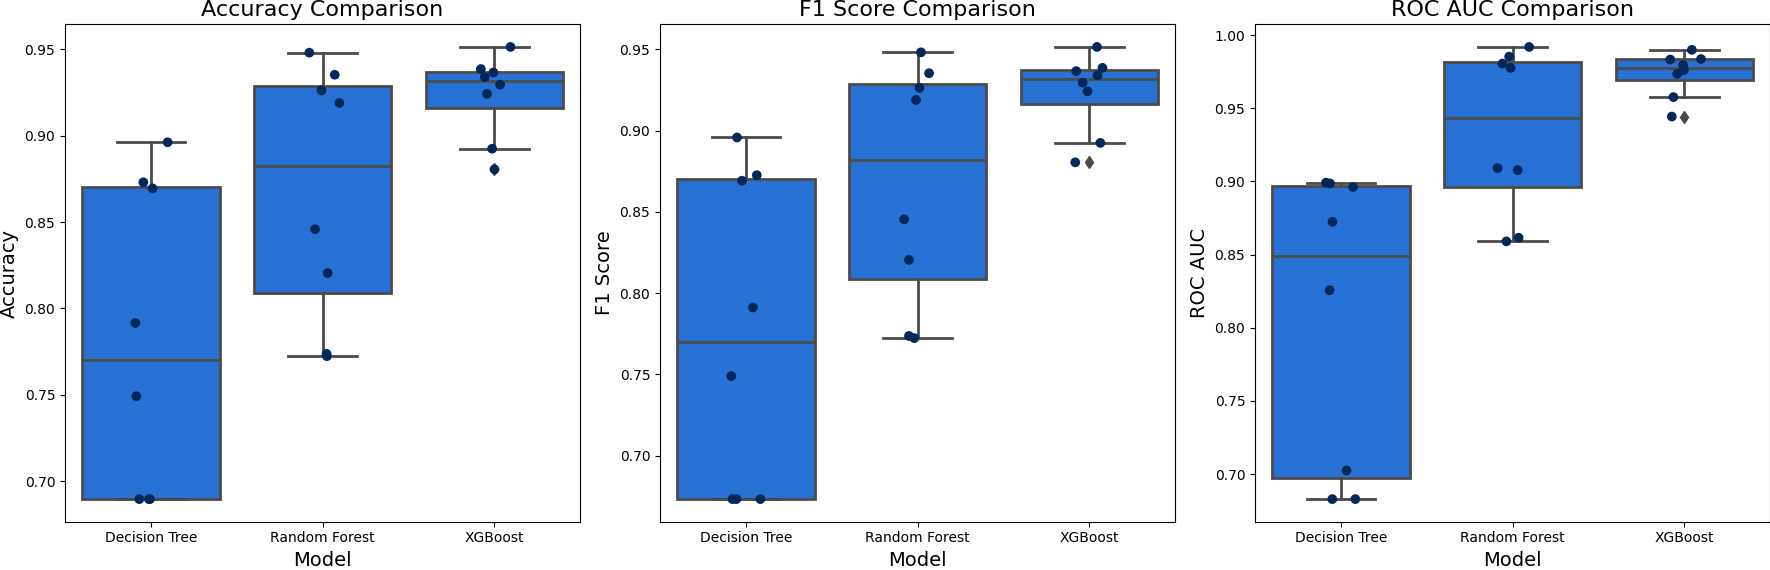
\includegraphics[width=460px]{ModelOptimization/box_plots_metrics.png}%
\caption{Boxplots of accuracy, f1, roc\_auc}%
\end{figure}

%
\subsection{Barplots of maximum values of metrics achievied by model}%
\label{subsec:Barplotsofmaximumvaluesofmetricsachieviedbymodel}%


\begin{figure}[h!]%
\centering%
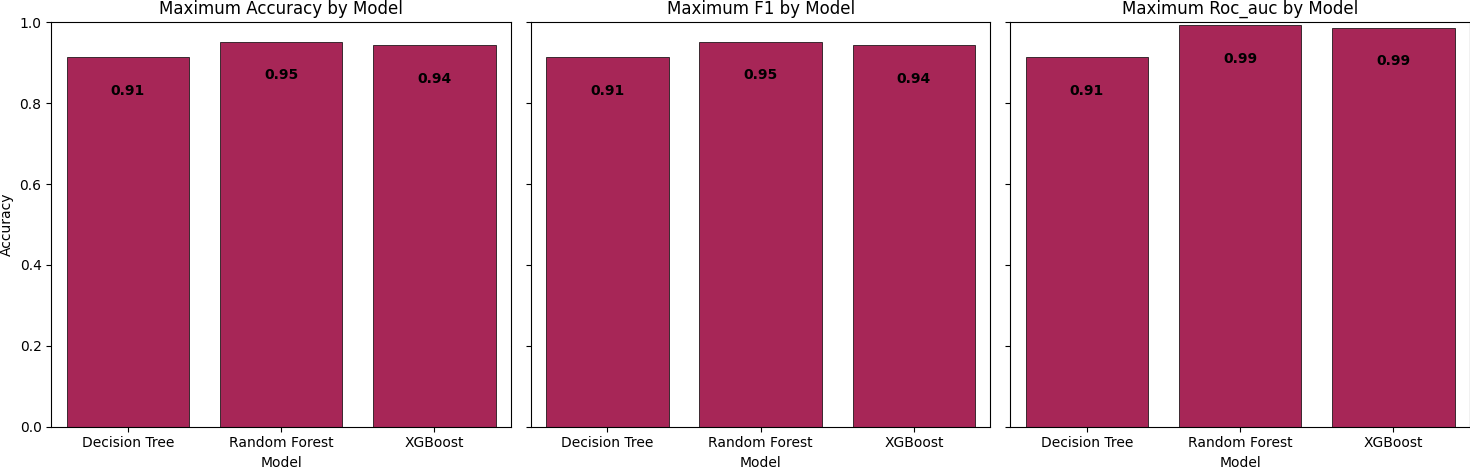
\includegraphics[width=460px]{ModelOptimization/barplots_max_metric.png}%
\caption{Barplots of maximum values of metrics achievied by model}%
\end{figure}

%
\newpage%
\section{Interpretabilty of the best models}%
\label{sec:Interpretabiltyofthebestmodels}%
Auto2class package defined the best model as the one that achievied the highest value of a metric, chosen by the user, or ROC AUC by default.%
In this case, the optimization process was aimed at maximizing%
\textbf{ Accuracy.}%
\\%
Do not forget, that after preprocessing, columns names have changed, because of transformations of categorical features.%
\subsection{The best XGBoost model Explanation}%
\label{subsec:ThebestXGBoostmodelExplanation}%


\begin{figure}[h!]%
\centering%
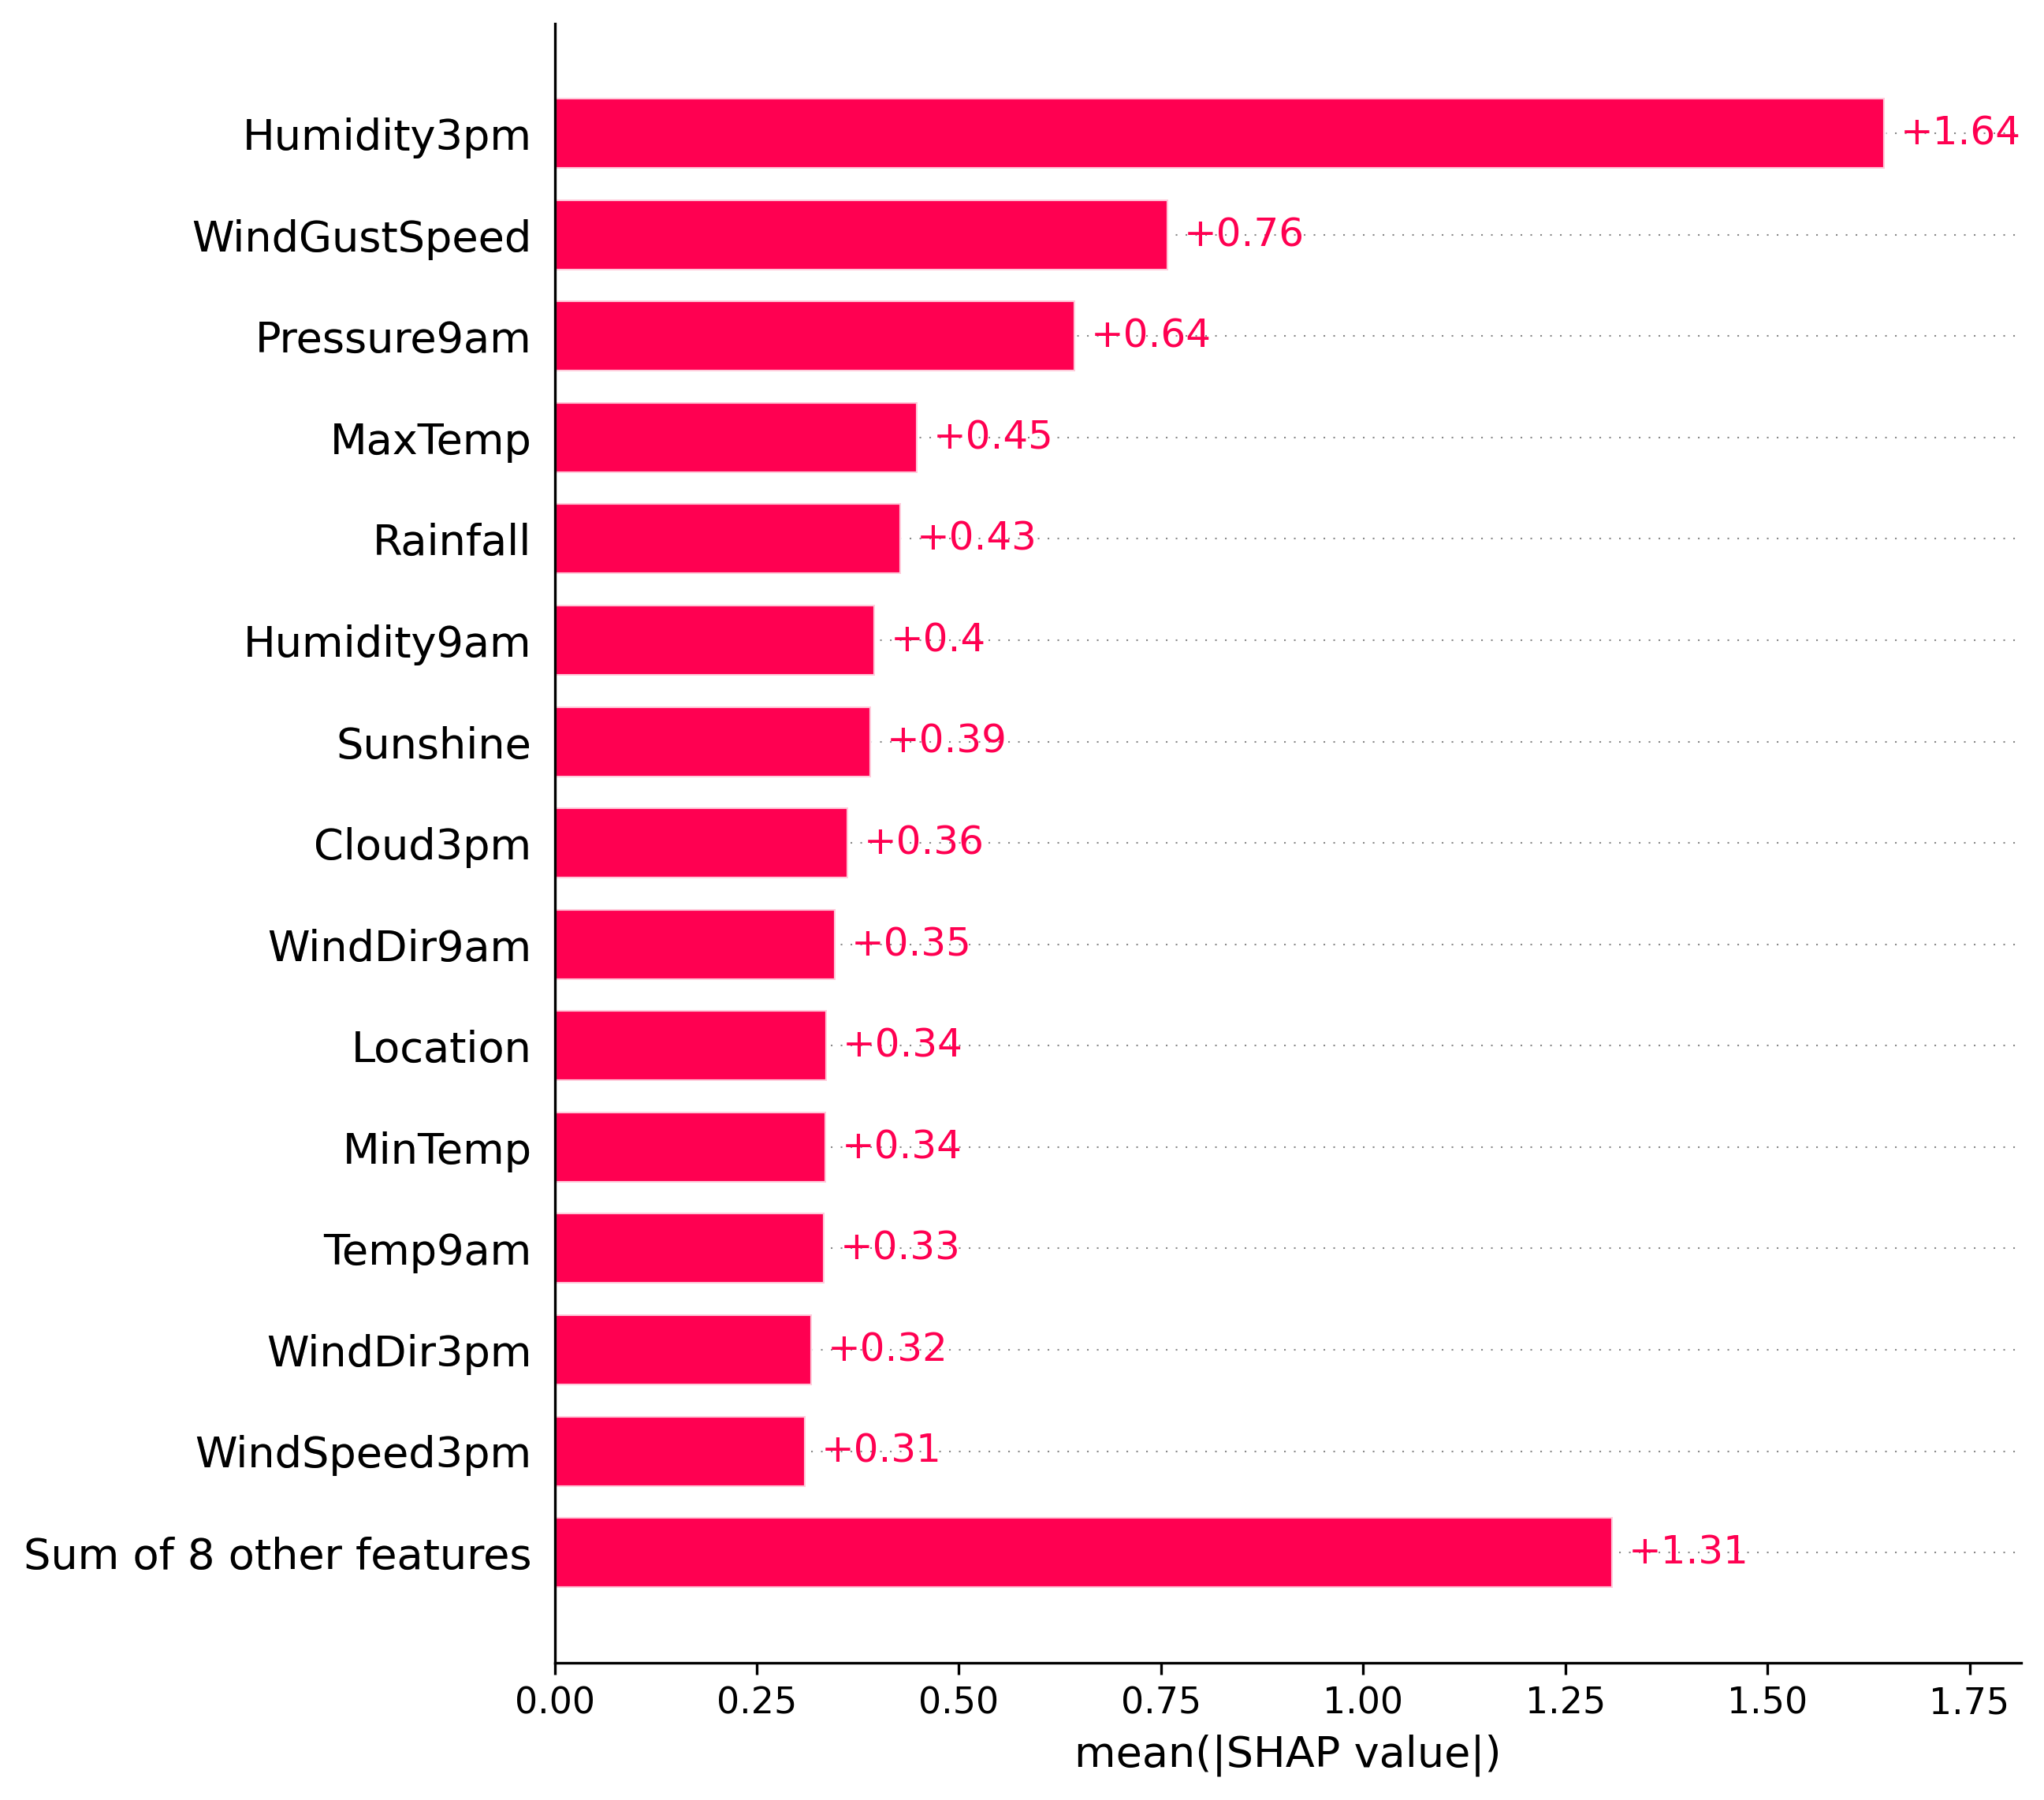
\includegraphics[width=350px]{XAI/XGBoost/global_feature_importance_shap.png}%
\caption{SHAP values for the best XGBoost model}%
\end{figure}

%


\begin{figure}[h!]%
\centering%
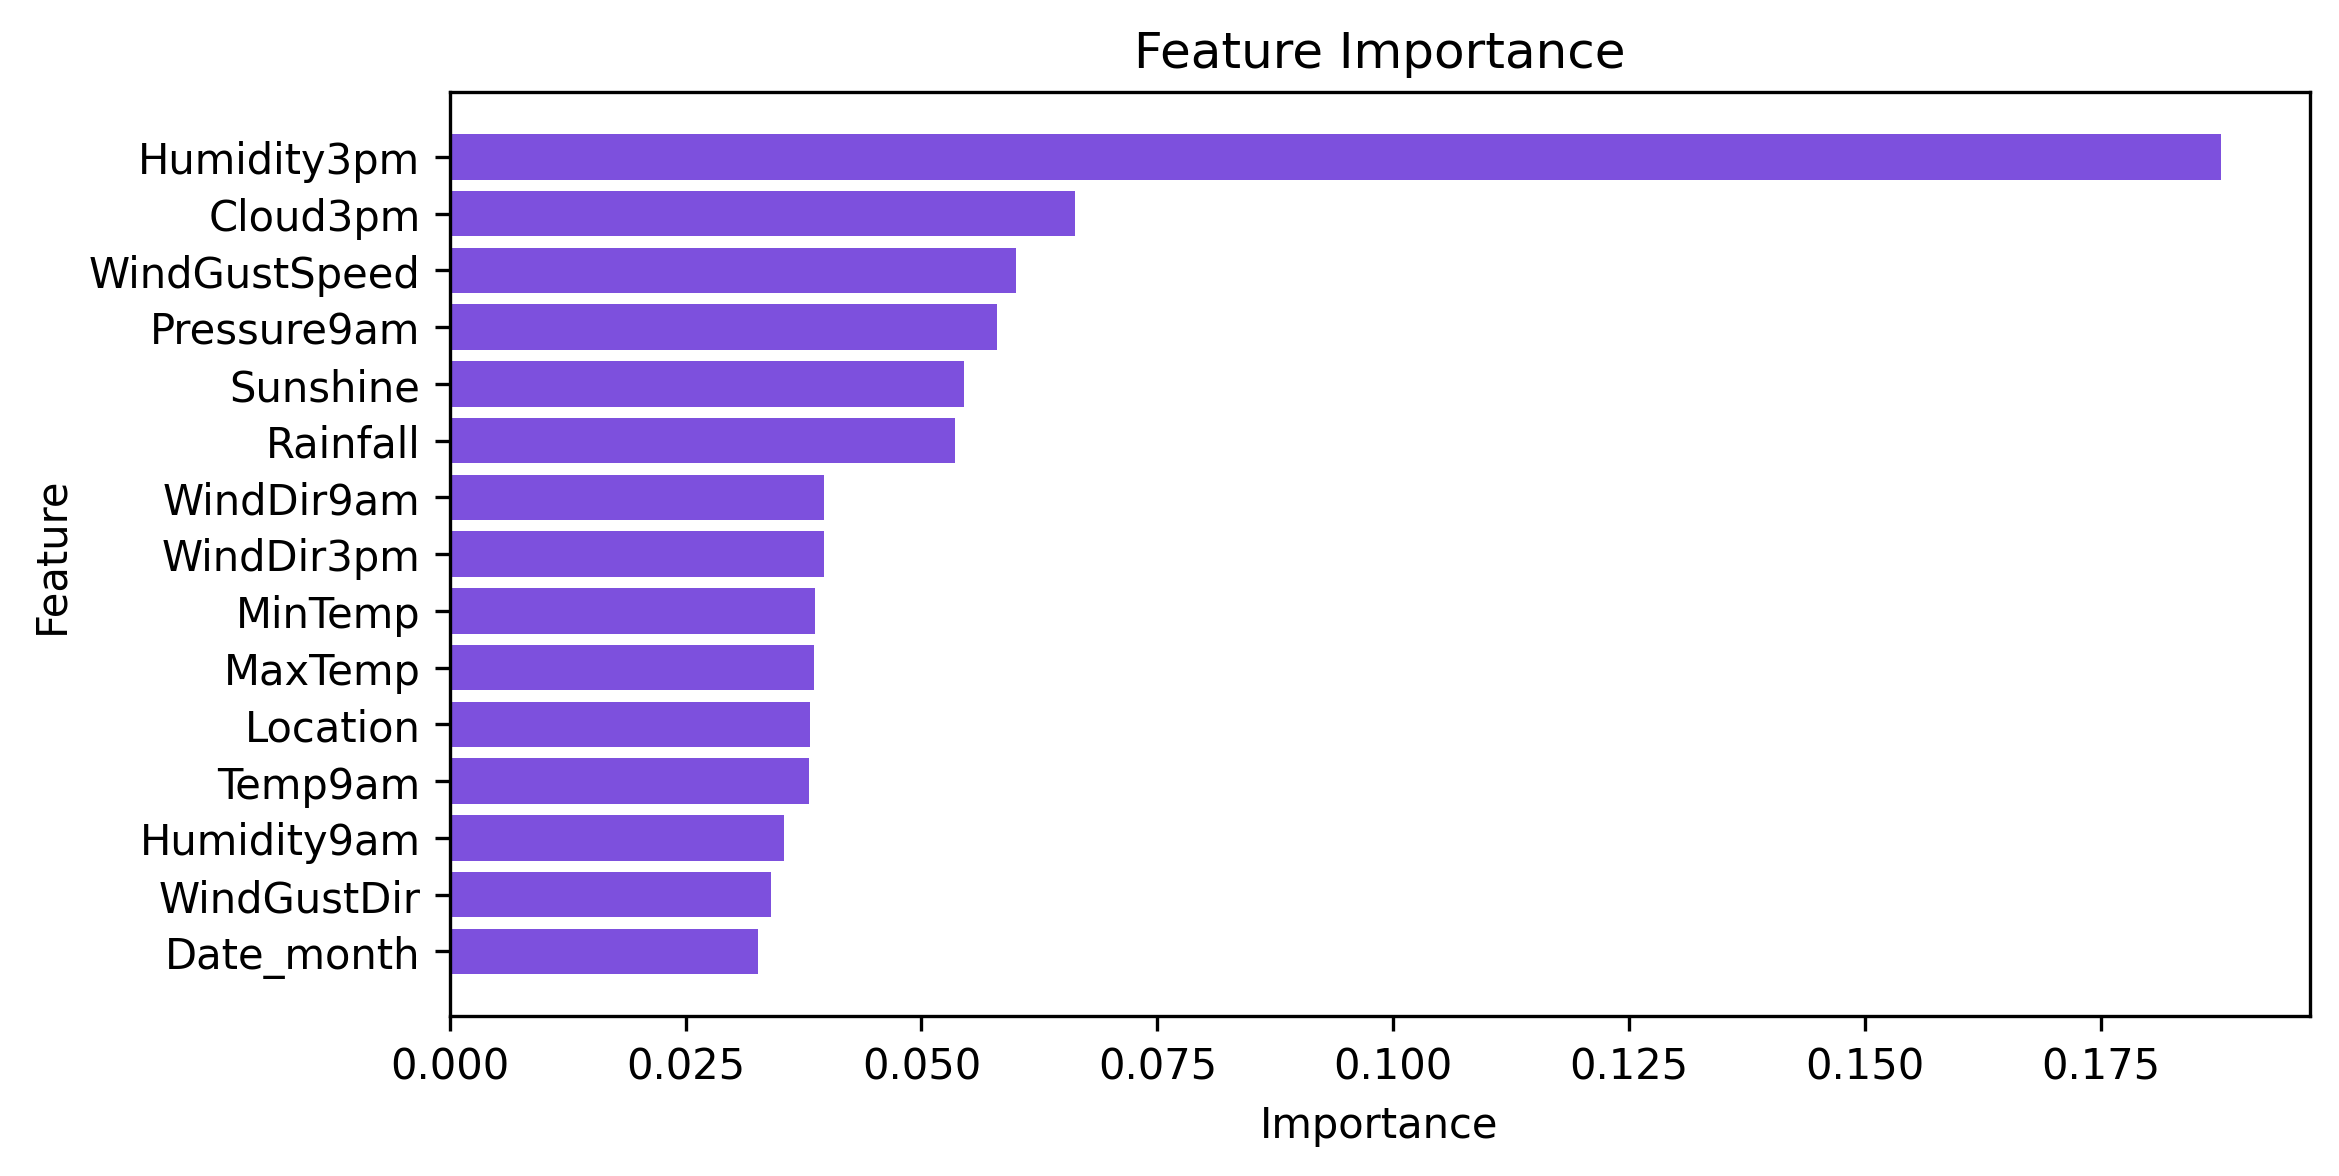
\includegraphics[width=350px]{XAI/XGBoost/feature_importance.png}%
\caption{Feature Importance for the best XGBoost model}%
\end{figure}

%


\begin{figure}[h!]%
\centering%
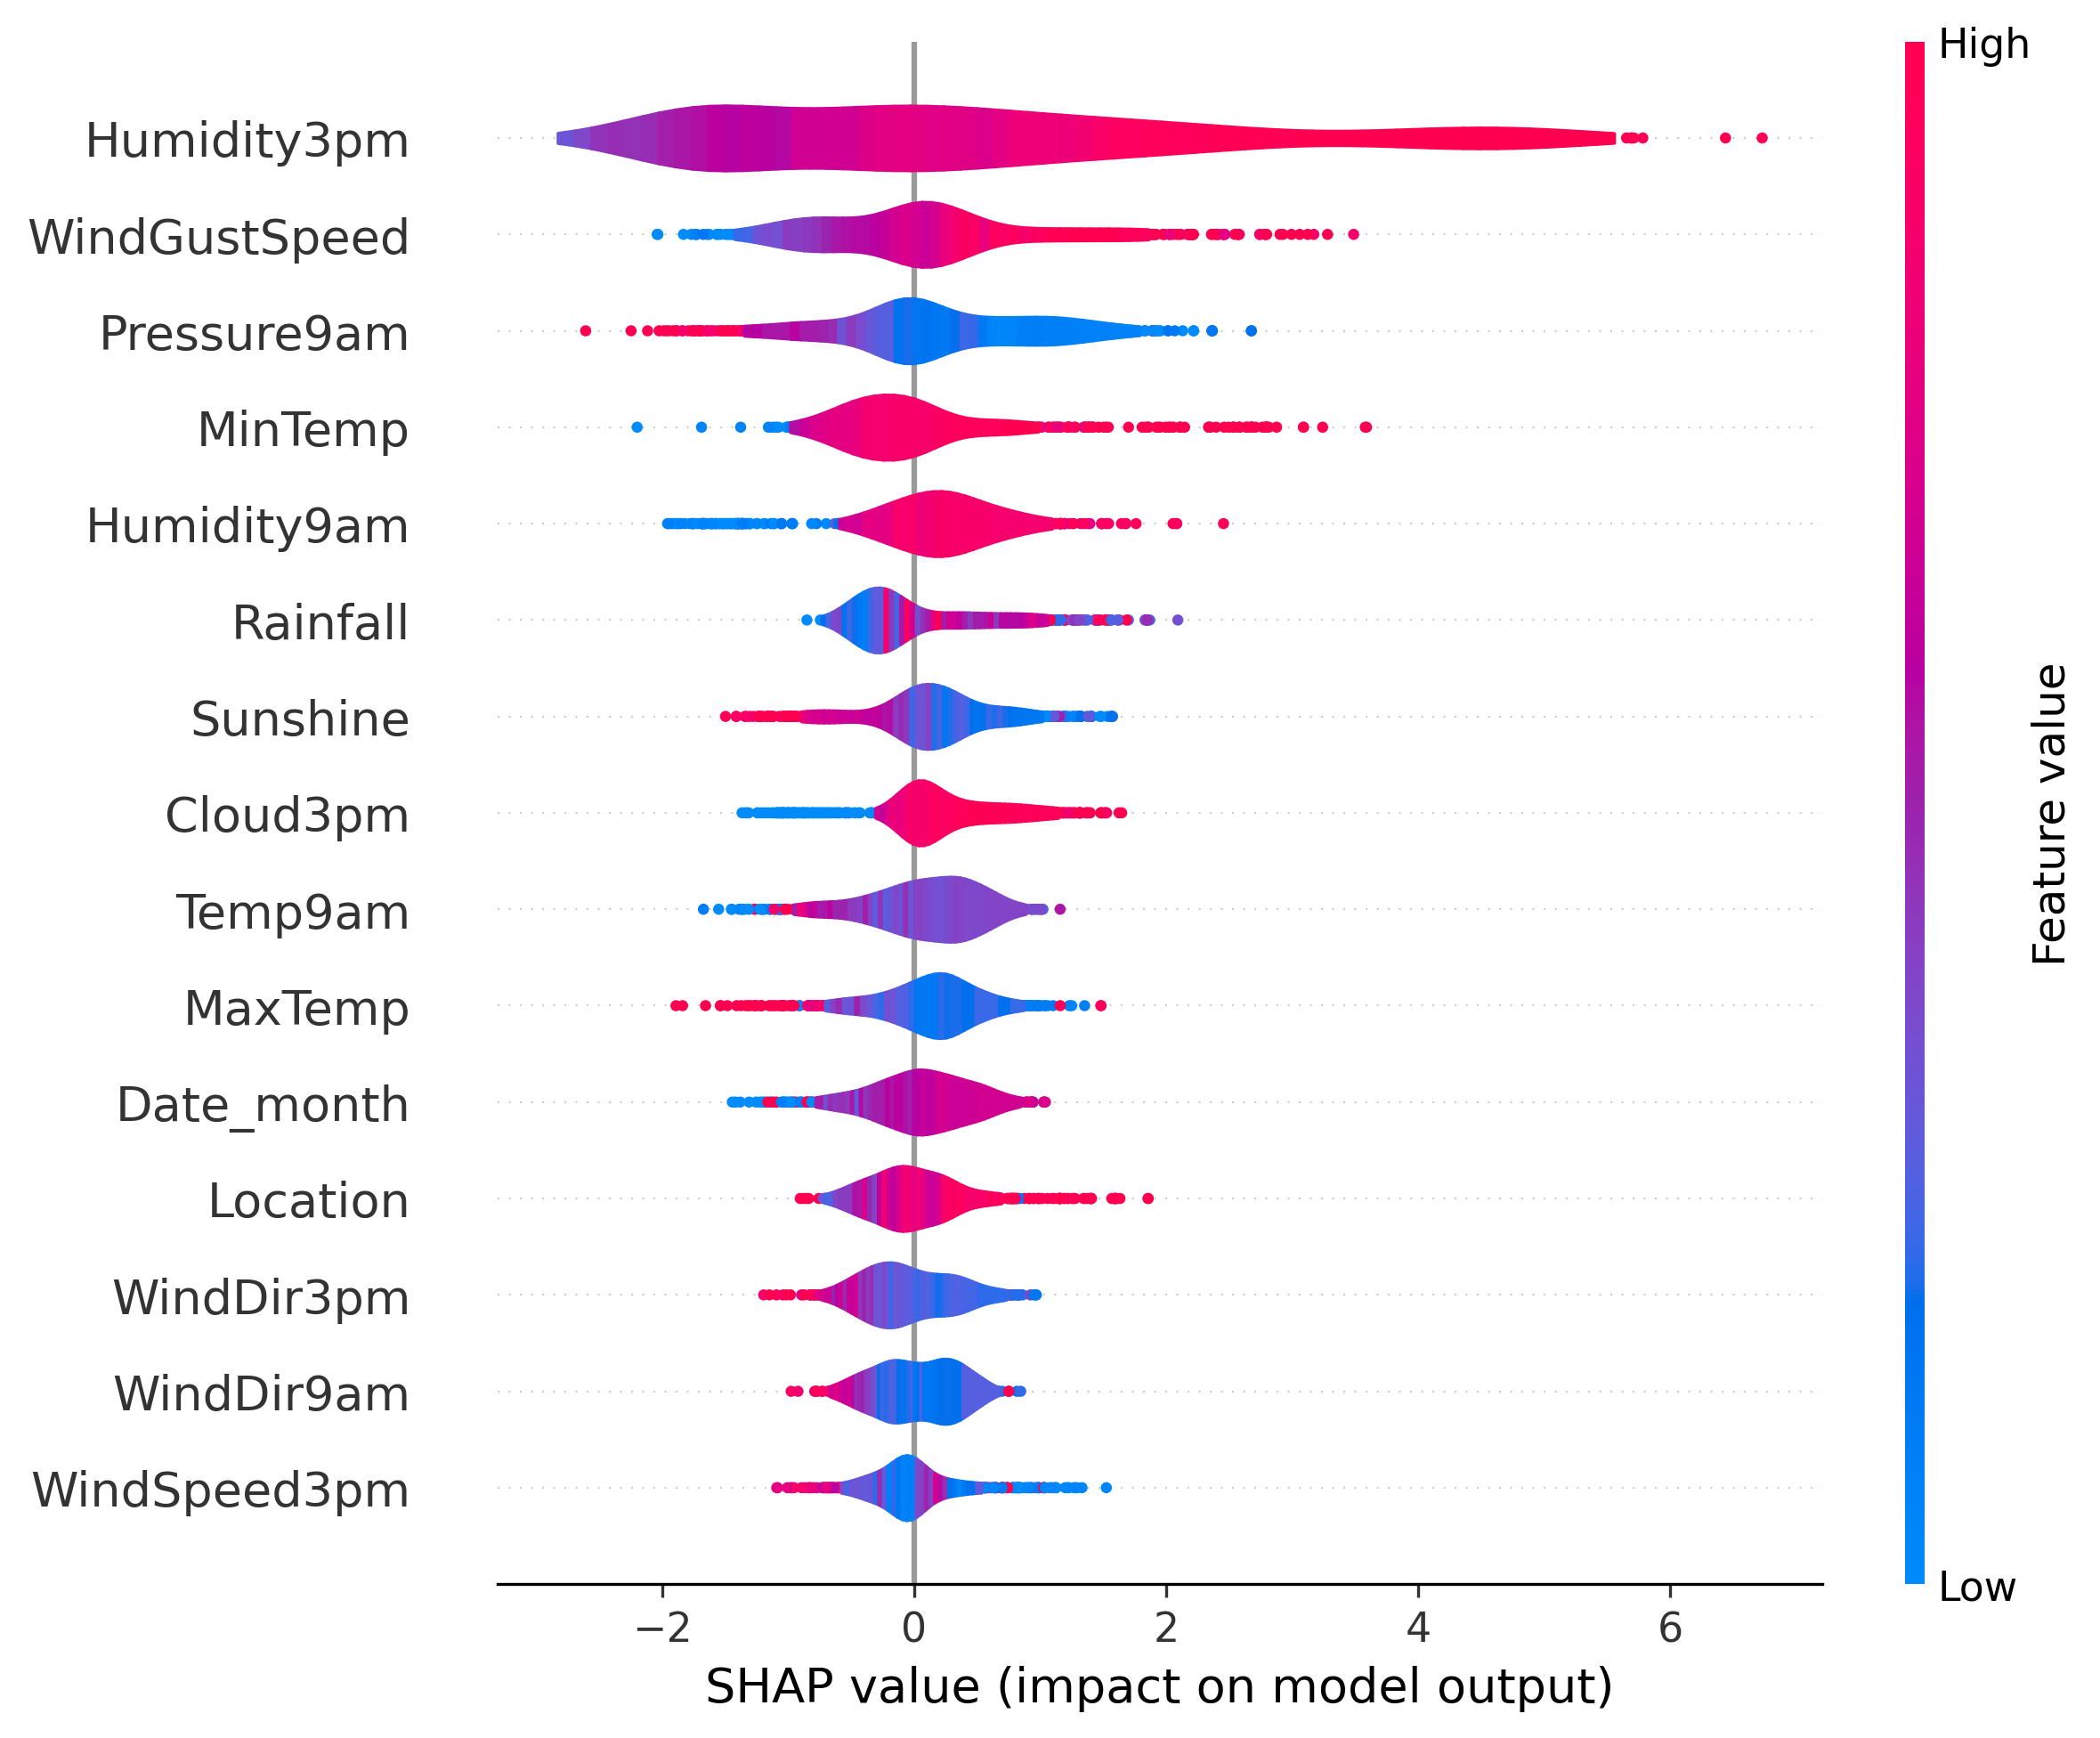
\includegraphics[width=400px]{XAI/XGBoost/violin_summary_plot_shap.png}%
\caption{Violin plot (SHAP) of impact on prediction for the best default XGBoost model}%
\end{figure}

%
\end{document}